\documentclass[11pt, a4paper]{article}
\usepackage{amsmath, amssymb, amsthm}
\usepackage{algorithm}
\usepackage{algpseudocode}
\usepackage{graphicx}
\usepackage{geometry}
\usepackage{hyperref}

\geometry{margin=1in}

\title{\textbf{The Power Method Algorithm}}
\author{}
\date{}

\newtheorem{theorem}{Theorem}
\newtheorem{remark}{Remark}

\begin{document}

\maketitle

\section{Introduction}

The \textbf{power method} (also called \textbf{power iteration}) is a classic iterative algorithm for computing the dominant eigenvalue and its corresponding eigenvector of a matrix. Given a square matrix $A \in \mathbb{R}^{n \times n}$, the method finds the eigenvalue with the largest absolute value, denoted $\lambda_1$, and its associated eigenvector $\mathbf{v}_1$.

\section{Algorithm Statement}

\subsection{Initialization}

\begin{itemize}
    \item Choose an initial vector $\mathbf{x}^{(0)} \in \mathbb{R}^n$ such that $\mathbf{x}^{(0)} \neq \mathbf{0}$. 
    \item Typically, $\mathbf{x}^{(0)}$ is chosen randomly or as $\mathbf{x}^{(0)} = (1, 1, \ldots, 1)^T$.
    \item Normalize: $\mathbf{x}^{(0)} \leftarrow \frac{\mathbf{x}^{(0)}}{\|\mathbf{x}^{(0)}\|}$ (optional but recommended).
    \item Set convergence tolerance $\epsilon > 0$ and maximum iterations $k_{\max}$.
\end{itemize}

\subsection{Iteration Step}

For $k = 0, 1, 2, \ldots$ until convergence:

\begin{enumerate}
    \item \textbf{Matrix-vector multiplication:}
    \begin{equation}
        \mathbf{y}^{(k+1)} = A\mathbf{x}^{(k)}
    \end{equation}
    
    \item \textbf{Normalization:}
    \begin{equation}
        \mathbf{x}^{(k+1)} = \frac{\mathbf{y}^{(k+1)}}{\|\mathbf{y}^{(k+1)}\|}
    \end{equation}
    where $\|\cdot\|$ denotes a vector norm (typically the Euclidean norm $\|\cdot\|_2$).
    
    \item \textbf{Eigenvalue estimate:} Compute the Rayleigh quotient
    \begin{equation}
        \lambda^{(k+1)} = \frac{(\mathbf{x}^{(k+1)})^T A \mathbf{x}^{(k+1)}}{(\mathbf{x}^{(k+1)})^T \mathbf{x}^{(k+1)}} = (\mathbf{x}^{(k+1)})^T A \mathbf{x}^{(k+1)}
    \end{equation}
    where the second equality holds if $\mathbf{x}^{(k+1)}$ is normalized.
    
    Alternatively, if the largest eigenvalue is known to be positive, one can use:
    \begin{equation}
        \lambda^{(k+1)} = \|\mathbf{y}^{(k+1)}\| = \|A\mathbf{x}^{(k)}\|
    \end{equation}
\end{enumerate}

\subsection{Convergence Criteria}

The iteration terminates when one of the following conditions is met:

\begin{enumerate}
    \item \textbf{Eigenvalue convergence:}
    \begin{equation}
        |\lambda^{(k+1)} - \lambda^{(k)}| < \epsilon
    \end{equation}
    
    \item \textbf{Eigenvector convergence:}
    \begin{equation}
        \|\mathbf{x}^{(k+1)} - \mathbf{x}^{(k)}\| < \epsilon
    \end{equation}
    or
    \begin{equation}
        \|\mathbf{x}^{(k+1)} + \mathbf{x}^{(k)}\| < \epsilon
    \end{equation}
    (the second condition accounts for sign ambiguity in eigenvectors).
    
    \item \textbf{Residual criterion:}
    \begin{equation}
        \|A\mathbf{x}^{(k+1)} - \lambda^{(k+1)}\mathbf{x}^{(k+1)}\| < \epsilon
    \end{equation}
    
    \item \textbf{Maximum iterations reached:} $k \geq k_{\max}$
\end{enumerate}

The most commonly used criterion is the eigenvalue convergence test (1) or the residual criterion (3).

\section{Formal Algorithm}

\begin{algorithm}
\caption{Power Method}
\begin{algorithmic}[1]
\Require Matrix $A \in \mathbb{R}^{n \times n}$, tolerance $\epsilon > 0$, max iterations $k_{\max}$
\Ensure Dominant eigenvalue $\lambda$ and eigenvector $\mathbf{x}$
\State Choose initial vector $\mathbf{x}^{(0)} \in \mathbb{R}^n$, $\mathbf{x}^{(0)} \neq \mathbf{0}$
\State $\mathbf{x}^{(0)} \leftarrow \mathbf{x}^{(0)} / \|\mathbf{x}^{(0)}\|$
\State $\lambda^{(0)} \leftarrow 0$
\For{$k = 0, 1, 2, \ldots, k_{\max}-1$}
    \State $\mathbf{y}^{(k+1)} \leftarrow A\mathbf{x}^{(k)}$
    \State $\mathbf{x}^{(k+1)} \leftarrow \mathbf{y}^{(k+1)} / \|\mathbf{y}^{(k+1)}\|$
    \State $\lambda^{(k+1)} \leftarrow (\mathbf{x}^{(k+1)})^T A \mathbf{x}^{(k+1)}$
    \If{$|\lambda^{(k+1)} - \lambda^{(k)}| < \epsilon$}
        \State \Return $\lambda^{(k+1)}, \mathbf{x}^{(k+1)}$
    \EndIf
\EndFor
\State \Return $\lambda^{(k_{\max})}, \mathbf{x}^{(k_{\max})}$ \Comment{Max iterations reached}
\end{algorithmic}
\end{algorithm}

\section{Convergence Properties}

\begin{theorem}[Convergence of Power Method]
Let $A \in \mathbb{R}^{n \times n}$ be diagonalizable with eigenvalues $\lambda_1, \lambda_2, \ldots, \lambda_n$ such that
\begin{equation}
    |\lambda_1| > |\lambda_2| \geq |\lambda_3| \geq \cdots \geq |\lambda_n|
\end{equation}
and corresponding eigenvectors $\mathbf{v}_1, \mathbf{v}_2, \ldots, \mathbf{v}_n$ that form a basis for $\mathbb{R}^n$. If the initial vector $\mathbf{x}^{(0)}$ has a nonzero component in the direction of $\mathbf{v}_1$, then the power method converges:
\begin{equation}
    \lambda^{(k)} \to \lambda_1 \quad \text{and} \quad \mathbf{x}^{(k)} \to \pm \mathbf{v}_1 \quad \text{as } k \to \infty
\end{equation}
\end{theorem}

\begin{remark}[Rate of Convergence]
The rate of convergence is determined by the ratio $\left|\frac{\lambda_2}{\lambda_1}\right|$. Specifically, the error decreases approximately as:
\begin{equation}
    \text{Error}^{(k)} \approx C \left|\frac{\lambda_2}{\lambda_1}\right|^k
\end{equation}
where $C$ is a constant depending on the initial vector. The convergence is \textbf{linear} with rate $\left|\frac{\lambda_2}{\lambda_1}\right|$.
\end{remark}

\begin{remark}[Conditions for Convergence]
The power method requires:
\begin{itemize}
    \item The matrix $A$ must have a unique dominant eigenvalue: $|\lambda_1| > |\lambda_2|$
    \item The initial vector must have a nonzero component in the direction of the dominant eigenvector
    \item The matrix need not be symmetric
\end{itemize}
\end{remark}

\section{Numerical Example}

Consider a $5 \times 5$ symmetric matrix with eigenvalues $\{10, 5, 3, 1, 0.5\}$. Applying the power method with a random initial vector demonstrates the convergence behavior shown in Figure~\ref{fig:convergence}.

\begin{figure}[h]
    \centering
    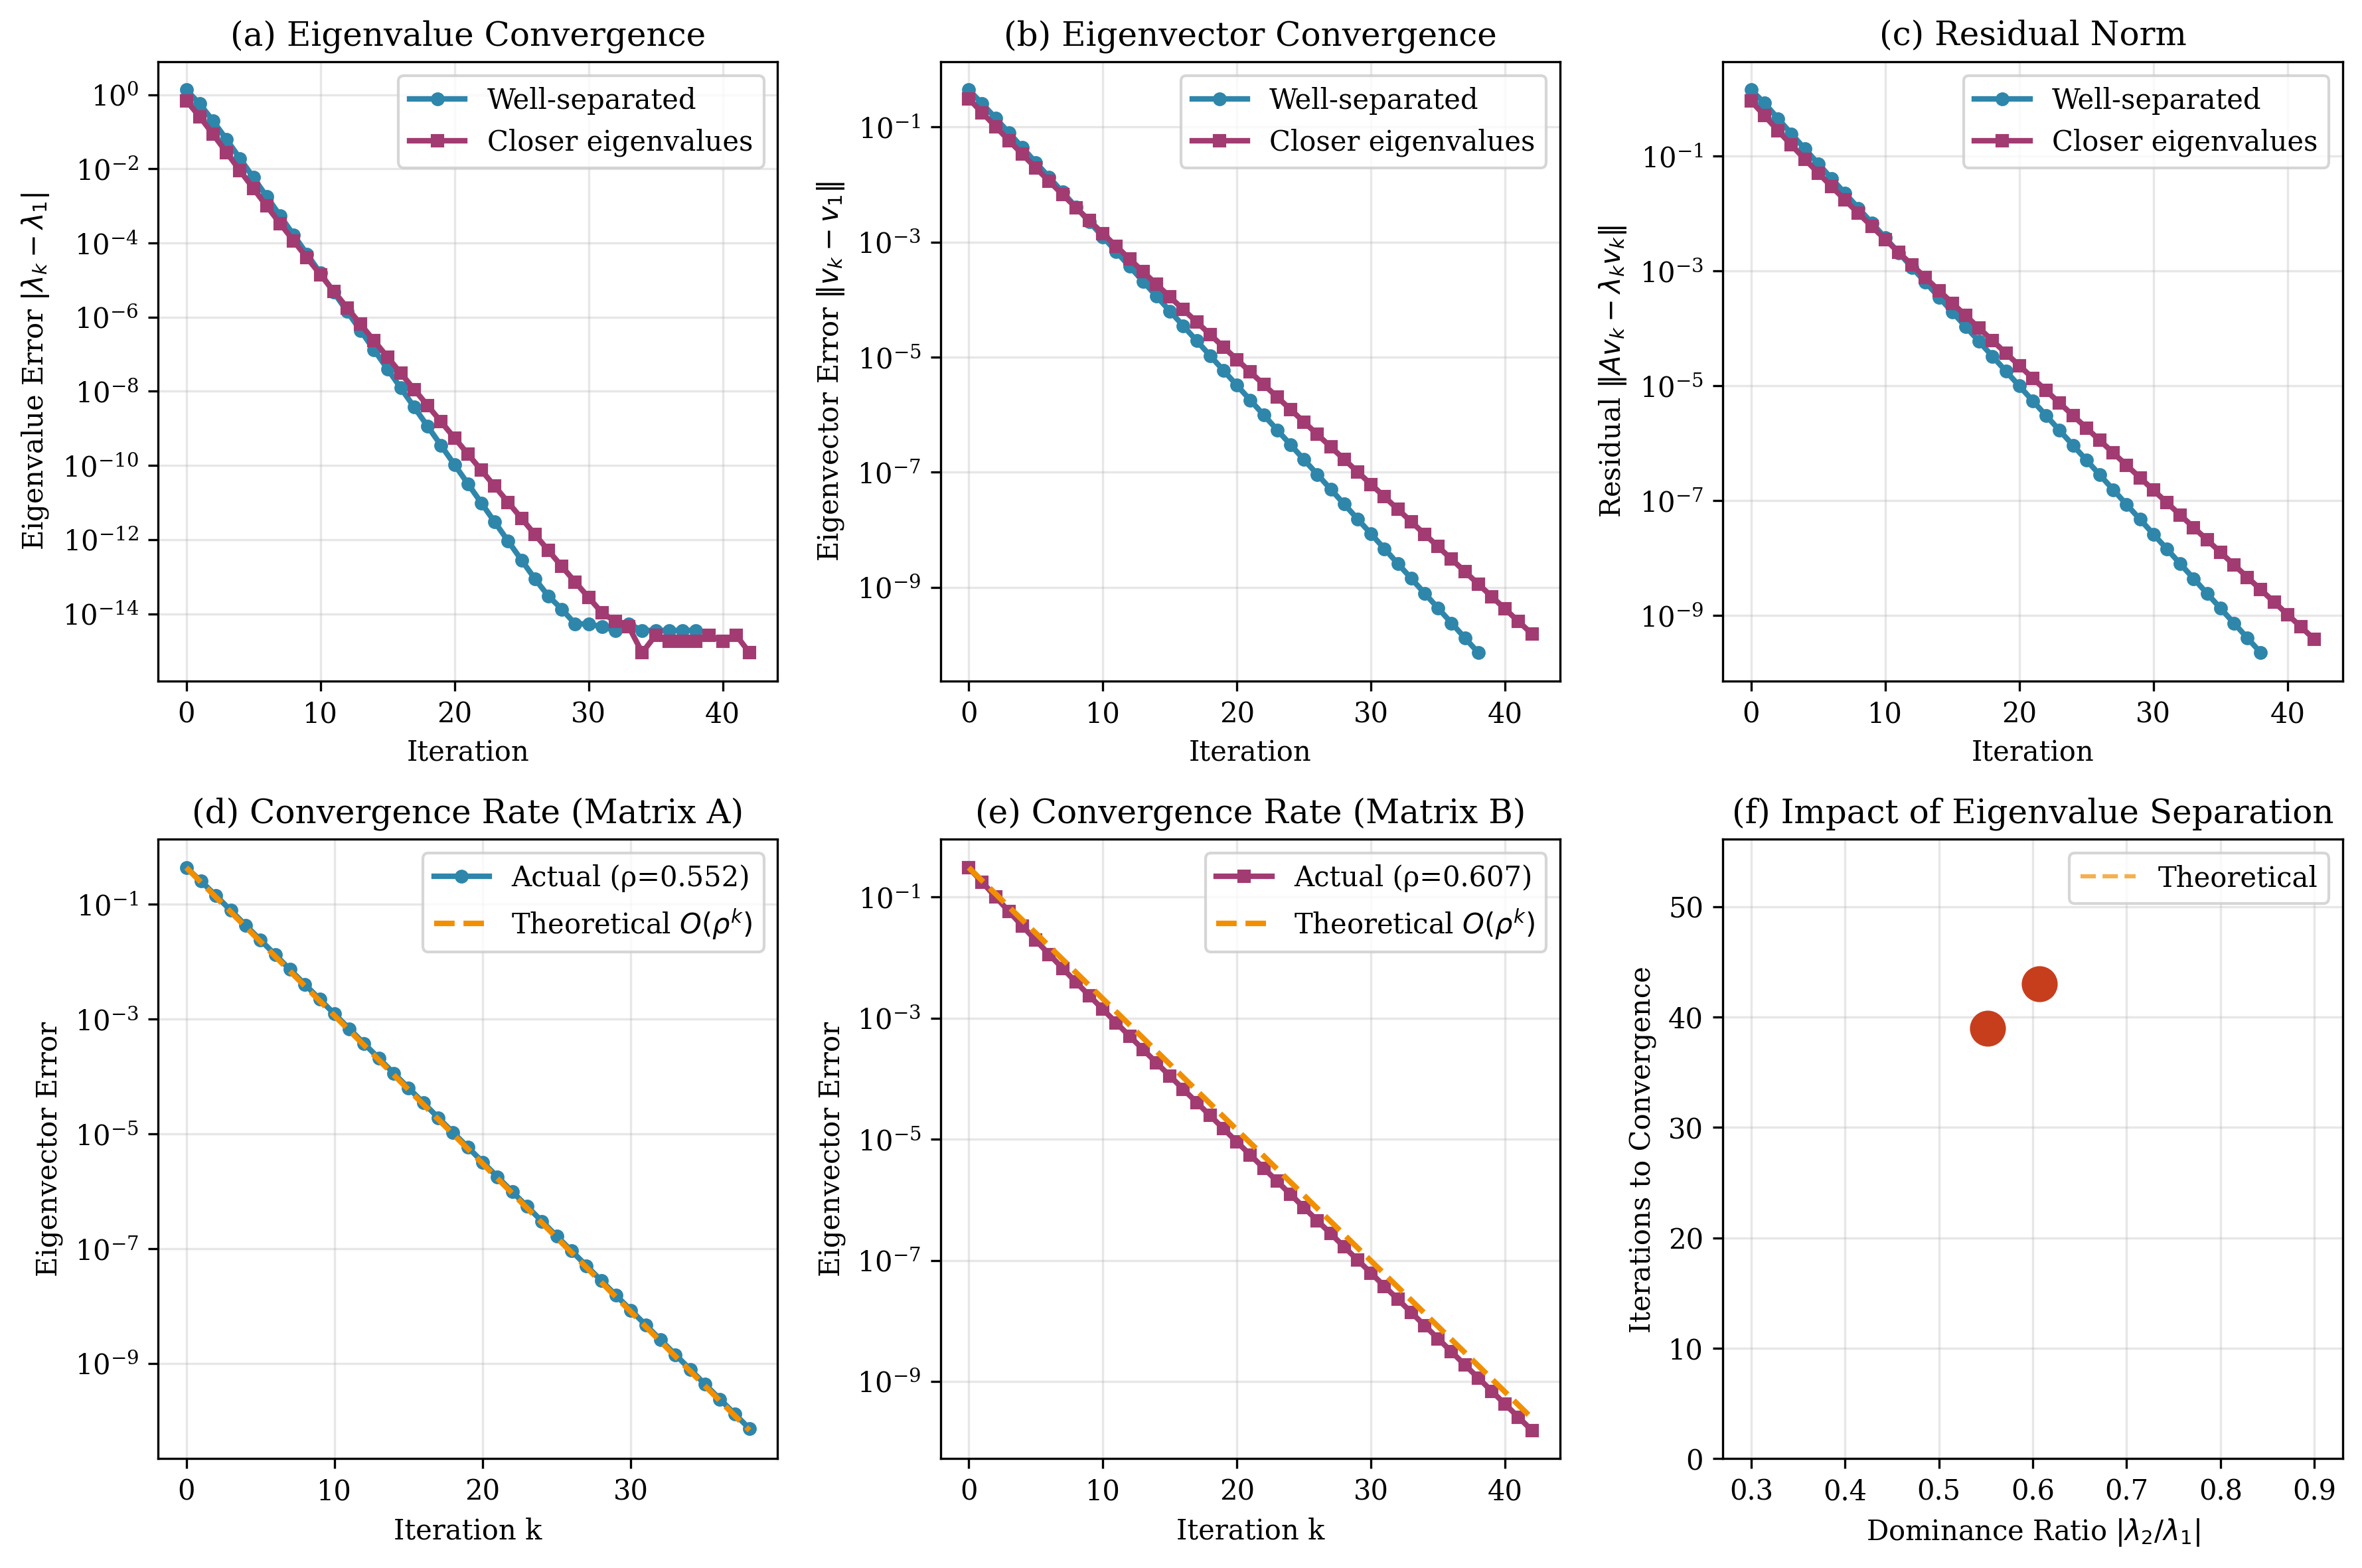
\includegraphics[width=0.8\textwidth]{power_method_convergence.png}
    \caption{Convergence of the power method. The error in the eigenvalue estimate decreases exponentially, exhibiting linear convergence with rate $|\lambda_2/\lambda_1| = 5/10 = 0.5$.}
    \label{fig:convergence}
\end{figure}

The method successfully computes the dominant eigenvalue $\lambda_1 = 10$ to high accuracy within a few dozen iterations.

\section{Variants and Extensions}

Several variants of the power method address specific computational needs:

\begin{itemize}
    \item \textbf{Inverse Power Method:} Applies the power method to $A^{-1}$ to find the smallest eigenvalue
    \item \textbf{Shifted Inverse Power Method:} Uses $(A - \mu I)^{-1}$ to find the eigenvalue closest to a shift $\mu$
    \item \textbf{Rayleigh Quotient Iteration:} Adaptive shift strategy for faster convergence
    \item \textbf{Orthogonal Iteration:} Generalizes to find multiple dominant eigenvalues and eigenvectors
\end{itemize}

\section{Computational Complexity}

Each iteration of the power method requires:
\begin{itemize}
    \item One matrix-vector multiplication: $O(n^2)$ operations for dense matrices, potentially $O(n)$ for sparse matrices
    \item One vector normalization: $O(n)$ operations
    \item One Rayleigh quotient computation: $O(n^2)$ operations for dense matrices
\end{itemize}

The total cost per iteration is $O(n^2)$ for dense matrices and potentially much less for sparse matrices, making the power method particularly attractive for large sparse eigenvalue problems.

\end{document}
